\documentclass[10pt,a4paper,twocolumn]{article}
% The following LaTeX packages must be installed on your machine: amsmath, authblk, bm, booktabs, caption, dcolumn, fancyhdr, geometry, graphicx, hyperref, latexsym, natbib
\input{151.dat}
\usepackage{gensymb}
\usepackage{amsthm}
\usepackage{float}
\usepackage{siunitx}
\usepackage{amssymb}
\usepackage{float}
\usepackage{enumerate}
\usepackage{listings}
\usepackage{mathtools}
\PassOptionsToPackage{hyphens}{url}\usepackage{hyperref}
\usepackage[none]{hyphenat}
\usepackage{physics}
\newcommand\ddfrac[2]{\frac{\displaystyle #1}{\displaystyle #2}}
%\renewcommand{\familydefault}{\sfdefault}


\begin{document}

\begin{titlepage}
\begin{center}
\vspace*{\fill}

\Huge{ Physics 151} \\
\normalsize{Crib Sheet \\
2nd semester, A.Y. 2018-19} \\

\qquad
\qquad

\normalsize{Kenneth V. Domingo \\
2015-03116 \\
28}

\vspace*{\fill}
\end{center}
\end{titlepage}

\tableofcontents

\clearpage

\setcounter{page}{1}

\section[P09 PS02 2.8 Work in a cyclic process]{P09 PS02 2.8}
Consider the cyclic process as described in Example 2.1.

\begin{figure}[htb]
	\centering
	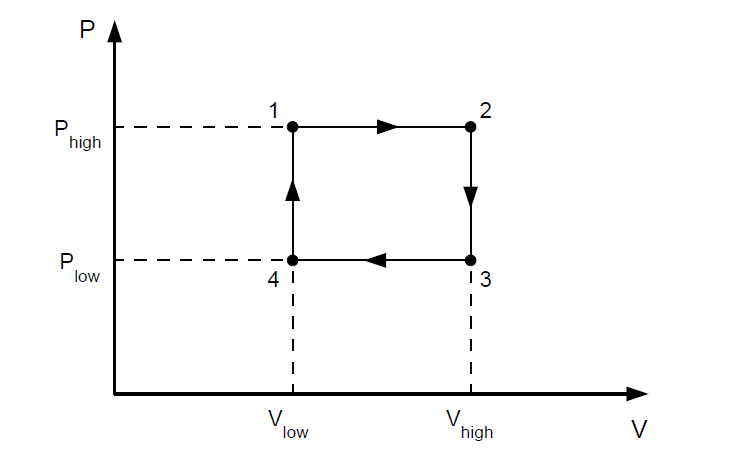
\includegraphics[width=0.75\linewidth]{work.png}
	\caption{Cyclic process for this problem.}
	\label{fig:2.8-cycle}
\end{figure}

\begin{enumerate}[(a)]
	\item Because the system was returned to its original pressure and volume, why is the net amount of work done on the system not zero?
	\item What would be the work done on the gas if the gas were taken from $1 \rightarrow 2 \rightarrow 3$ and then back to 1 along the diagonal path connecting 3 and 1?
\end{enumerate}


\section{P10 PS02 2.13}
In Example 2.1 we showed that the net work done on the gas in the cyclic process shown in Figure \ref{fig:2.8-cycle} is nonzero. Assume that the gas is ideal with N particles and calculate the energy transfer by heating in each step of the process. Then explain why the net work done on the gas is negative and show that the net change of the internal energy is zero.

From Example 2.1, the net work done on a gas in a cyclic process was determined to be nonzero, with a value of

\begin{equation}\label{oldanswer}
	W_{net} = -\left( P_{high} - P_{low} \right) \left( V_{high} - V_{low} \right)
\end{equation}

Assuming an ideal gas with $N$ particles, the energy transfer due to heating for each step in the process is as follows:

\begin{align}
	Q_{1 \rightarrow 2} = -Q_{3 \rightarrow 4} & = \int_{T_1}^{T_2} c_P \textrm{ d}T \\
	& = \nu c_P \int_{T_1}^{T_2} \textrm{ d}T \\
	& = \nu c_P \left( T_2 - T_1 \right) \\
	& = \nu c_P \Delta T \label{eq:isobaric} \\
	Q_{2 \rightarrow 3} = -Q_{4 \rightarrow 1} & = \int_{T_1}^{T_2} c_V \textrm{ d}T \\
	& = \nu c_V \int_{T_1}^{T_2} \textrm{ d}T \\
	& = \nu c_V \left( T_2 - T_1 \right) \\
	& = \nu c_V \Delta T \label{eq:isochoric}
\end{align}

Recalling the ideal gas equation,

\begin{eqnarray}
	PV = \nu RT \label{eq:idealgas} \\
	T = \frac{PV}{\nu R} \label{eq:idealtemp}
\end{eqnarray}

The net energy transfer due to heating is

\begin{equation}\label{eq:totalwork}
	W_{net} = Q_{1 \rightarrow 2} + Q_{2 \rightarrow 3} + Q_{3 \rightarrow 4} + Q_{4 \rightarrow 1}
\end{equation}

Plugging \eqref{eq:idealtemp} into each of the equations in \eqref{eq:isobaric} and \eqref{eq:isochoric}, we have

\begin{align}
	Q_{1 \rightarrow 2} & = \nu c_P P_{high} \frac{V_{high} - V_{low}}{\nu R} \label{eq:Q12plug} \\
	Q_{2 \rightarrow 3} & = \nu c_V V_{high} \frac{P_{low} - P_{high}}{\nu R} \label{eq:Q23plug} \\
	Q_{3 \rightarrow 4} & = \nu c_P P_{low} \frac{V_{low} - V_{high}}{\nu R} \label{eq:Q34plug} \\
	Q_{4 \rightarrow 1} & = \nu c_V V_{low} \frac{P_{high} - P_{low}}{\nu R} \label{eq:Q41plug}
\end{align}

Simplifying equations \eqref{eq:Q12plug} through \eqref{eq:Q41plug} and summing them as in \eqref{eq:totalwork}, we have

\begin{align}
	Q_{net} & = c_P P_{high} \frac{V_{high} - V_{low}}{R} \nonumber \\
	& - c_V V_{high} \frac{P_{high} - P_{low}}{R} \nonumber \\
	& - c_P P_{low} \frac{V_{high} - V_{low}}{R} \nonumber \\
	& + c_V V_{low} \frac{P_{high} - P_{low}}{R}
\end{align}
\begin{align}
	Q_{net} & = \frac{c_P}{R} \left( P_{high} - P_{low} \right) \left( V_{high} - V_{low} \right) \nonumber \\
	& -\frac{c_V}{R} \left( P_{high} - P_{low} \right) \left( V_{high} - V_{low} \right) \label{eq:Wnetplug}
\end{align}

Recall that for an ideal gas,

\begin{eqnarray}
	c_P = \frac{5}{2} R \label{eq:idealcp} \\
	c_V = \frac{3}{2} R \label{eq:idealcv}
\end{eqnarray}

Plugging these into \eqref{eq:Wnetplug},

\begin{align}
	Q_{net} & = \frac{5}{2} R \frac{1}{R} \left( P_{high} - P_{low} \right) \left( V_{high} - V_{low} \right) \nonumber \\
	& -\frac{3}{2} R \frac{1}{R} \left( P_{high} - P_{low} \right) \left( V_{high} - V_{low} \right) \label{eq:Wnetideal}
\end{align}

Which gives us the expected relation of $Q_{net} = -W_{net}$ (negative because in a cyclic process, there is no change in internal energy; the work done is equal to the heat added):

\begin{equation}\label{eq:answer}
	Q_{net} = \left( P_{high} - P_{low} \right) \left( V_{high} - V_{low} \right)
\end{equation}

From the first thermodynamic law,

\begin{equation}\label{eq:1stlaw}
	\Delta E = Q + W
\end{equation}

Plugging equations \eqref{oldanswer} and \eqref{eq:answer} into this, we have

\begin{equation}\label{eq:energychange}
	\Delta E = 0
\end{equation}

\section{P11 PS03 2.15}
Use (2.44) and the ideal gas pressure equation of state in (2.8) to show that in a quasistatic adiabatic processes $P$ and $V$ are related as

\begin{equation}
	PV^\gamma = \textrm{constant}
\end{equation}

Also show that $T$ and $P$ are related as

\begin{equation}
	TP^{(1-\gamma)/\gamma} = \textrm{constant}
\end{equation}

The given equations are:

\begin{eqnarray}
	TV^{\gamma-1} = C \label{eq:given1} \\
	PV = \nu RT \label{eq:idealgaslaw}
\end{eqnarray}

Isolating $T$ in \eqref{eq:idealgaslaw},

\begin{equation}
	T = \frac{PV}{\nu R} \label{eq:idealgastemp}
\end{equation}

Plugging this into \eqref{eq:given1},

\begin{align}
	\frac{PV}{\nu R} V^{\gamma - 1} = C \nonumber \\
	PV^{\gamma} = C\nu R = C
\end{align}

Therefore,

\begin{equation}\label{eq:answer1}
\boxed{	PV^\gamma = \textrm{constant}}
\end{equation}

Similarly, isolating $V$ from \eqref{eq:idealgaslaw},

\begin{equation}\label{eq:idealgasvol}
	V = \frac{\nu RT}{P}
\end{equation}

Plugging this into \eqref{eq:answer1},

\begin{align}
	P\left( \frac{\nu RT}{P} \right)^\gamma & = C \nonumber \\
	\left( \nu RT \right)^\gamma P^{1-\gamma} & = C \nonumber \\
	T^\gamma P^{1-\gamma} & = \frac{C}{\left( \nu R \right)^\gamma} \nonumber \\
	T^\gamma P^{1-\gamma} & = D
\end{align}

Raising both sides to $1/\gamma$,

\begin{eqnarray}
	\left( T^\gamma P^{1-\gamma} \right)^{\frac{1}{\gamma}} = D^{\frac{1}{\gamma}} \nonumber \\
\boxed{	TP^{(1 - \gamma)/\gamma} = \textrm{constant}} \label{eq:answer2}
\end{eqnarray}

\section[P12 PS03 2.17 Compression of air]{P12 PS03 2.17}
\begin{enumerate}[(a)]

\item Air initially at $20^\circ$C is compressed by a factor of 15. Assuming adiabatic conditions, $V_i/15 = V_f$, $T_i = 293$K, and $\gamma = 1.4$,

\begin{eqnarray}
	TV^{\gamma -1} = C \label{eq:adiabatic} \\
	T_i V_i^{\gamma-1} = T_f V_f^{\gamma - 1} \nonumber \\
	293 V_i^{0.4} = T_f \left( \frac{V_i}{15} \right)^{0.4} \nonumber \\
	293 = T_f \left(\frac{1}{15}\right)^{0.4} \nonumber \\
	T_f = 293 \left( \frac{1}{15} \right)^{-0.4} \nonumber \\
	\boxed{T_f = 866\textrm{ K}} \label{eq:answer1}
\end{eqnarray}

Assuming air behaves like an ideal gas,

\begin{eqnarray}
	\frac{P_i V_i}{T_i} = \frac{P_f V_f}{T_f} \\
	\frac{P_i}{293}\frac{V_f}{15} = \frac{P_f V_f}{866} \nonumber \\
	\frac{P_i}{(293)(15)} = \frac{P_f}{866} \nonumber \\
	\boxed{P_i \approx 5 P_f} \label{eq:answer2}
\end{eqnarray}

	\item If the compression is isothermal,

\begin{eqnarray}
	P_i V_i = P_f V_f \\
	\boxed{P_i = 15 P_f} \label{eq:answer3}
\end{eqnarray}

	\item The pressure increases more with adiabatic compression.

\end{enumerate}

\section[P13 PS03 2.18 Work done in a quasistatic adiabatic process]{P13 PS03 2.18}

\begin{enumerate}[(a)]

\item Use the result that we derived in (2.53) to obtain the alternative form (2.54).

From the given equations,

\begin{eqnarray}
	W = C_V \left( T_2 - T_1 \right) \label{eq:workvol} \\
	PV = \nu RT \label{eq:idealgas} \\
	C_V = \frac{3}{2} \nu k_B \label{eq:volenergy}
\end{eqnarray}

Plugin \eqref{eq:idealgas} and \eqref{eq:volenergy} into \eqref{eq:workvol}:

\begin{align}
	W & = \frac{3}{2} \nu k_B \left( \frac{P_2 V_2}{\nu k_B} - \frac{P_1 V_1}{\nu k_B} \right) \nonumber \\
	& = \frac{3}{2} \left( P_2 V_2 - P_1 V_1 \right)
\end{align}

Since $\gamma = \frac{5}{3}$ for monatomic ideal gas,

\begin{align}
	W & = \frac{\left( P_2 V_2 - P_1 V_1 \right)}{\frac{2}{3}} \nonumber \\
	& = \frac{\left( P_2 V_2 - P_1 V_1 \right)}{\frac{5}{3} - \frac{3}{3}} \nonumber \\
	\Aboxed{ W & = \frac{\left( P_2 V_2 - P_1 V_1 \right)}{\gamma - 1}} \label{eq:answer1}
\end{align}

\item Show that another way to derive (2.54) is to use the relations (2.14) and (2.46).

From the given equations,

\begin{eqnarray}
	PV^\gamma = C \label{eq:constant} \\
	W = -\int_{V_1}^{V_2} P(T,V) \dd{V} \label{eq:workint}
\end{eqnarray}

Isolate $P$ from \eqref{eq:constant} and plug into \eqref{eq:workint}:

\begin{align}
	W &= -\int_{V_1}^{V_2} C V^{-\gamma} \dd{V} \nonumber \\
	& = -C \frac{V^{1 - \gamma}}{1 - \gamma} \bigg|_{V_1}^{V_2} \nonumber \\
	& = \frac{1}{\gamma - 1}\left( CV_2^{1-\gamma} - CV_1^{1-\gamma} \right) \nonumber \\
	& = \frac{1}{\gamma - 1}\left( CV_2^{-\gamma}V_2 - CV_1^{-\gamma}V_1 \right)
\end{align}

From \eqref{eq:constant},

\begin{equation}
	P = CV^{-\gamma}
\end{equation}

Therefore,

\begin{equation}\label{eq:answer2}
\boxed{	W = \frac{1}{\gamma - 1} \left( P_2 V_2 - P_1 V_1 \right) }
\end{equation}

\end{enumerate}

\end{document}